\documentclass[a4paper,12pt]{article}

\usepackage[table]{xcolor}%TABLAS
\usepackage[hypcap=false, font=small, justification=centering, labelfont=bf]{caption}
\usepackage{multicol}%poder colocar columnas
\usepackage{amsmath} %formulas
\usepackage{amssymb} %simbolos
\usepackage{amsfonts} 
\usepackage{xcolor}%cambiar el color del texto
\usepackage[utf8]{inputenc} %facilitar la escritura en español 
\usepackage{graphicx}% figuras
\graphicspath{{./Fotos/}}
\usepackage[spanish,es-tabla]{babel} %tipografia del idioma
\usepackage{booktabs} %toprule, midrule, etc.
\usepackage{multirow}
\usepackage{hyperref}%crear e insertar links
\providecommand{\abs}[1]{\lvert#1\rvert}%poner valor absoluto
%\usepackage{biblatex}%bibliografia automatica apartir de base bib

%\usepackage{array}
%\usepackage{verbatim}%escribir sin codigos y comentarios multilinea
%\usepackage{siunitx}%unidades del sistema internacional
%\usepackage{subcaption}%leyendas en objetos que tienen su leyenda
%\usepackage{fancyhdr}%personalizar encabezado y pie de pagina
%\usepackage{longtable}%crear tablas largas
%\usepackage{colortbl}
%\usepackage{blindtext}%texto de relleno
%\usepackage{grffile}
%\usepackage{mathrsfs}
%\usepackage{siunitx}
%\usepackage{soul}%subrayar

\newenvironment{Figure}
  {\par\medskip\noindent\minipage{\linewidth}}
  {\endminipage\par\medskip}

\usepackage{anysize}
\marginsize{2cm}{2cm}{1cm}{2cm}

\setlength\columnsep{18pt}
\setlength\parskip{4pt} \setlength\parindent{0in}

\title{Formación de imágenes por refracción con lentes \\ 
\medskip \large Universidad Nacional de Tucumán - Laboratorio IV}
\author{Iker Algañaraz, May Juarez F., Gastón A. Lozano S., Belén N. Paz}
\date{}

\begin{document}

\maketitle

\section*{Resumen}

    En este informe se comprueba la aplicabilidad del modelo de lente delgada en nuestro sistema, tanto para lentes convergentes como para lentes divergentes. Además, se detalla el control de los supuestos del modelo con aberraciones de esfericidad y cromáticas. Se explora también una aplicación de un sistema de lentes, que son los telescopios refractores.

\medskip

\begin{multicols*}{2}

\section*{Introducción}

    La formación de imágenes con lentes es un fenómeno óptico fundamental que desempeña un papel crucial en una amplia variedad de aplicaciones como en la fotografía, la medicina y la astronomía. 
    %Este informe se sumerge en los principios matemáticos y físicos que rigen la formación de imágenes con lentes.
    En este informe tratamos el marco teórico necesario para comprender el modelo de lente delgada, la manera de corroborar sus supuestos y verificar la aplicabilidad del modelo a un sistema experimental.

\section*{Marco teórico}

    Llamamos lentes a medios transparentes limitados por superficies esféricas de curvaturas variables. Las lentes delgadas son un caso especial de lentes en el que su grosor es despreciable en comparación a las longitudes asociadas con sus propiedades ópticas, tales como la distancia objeto, la distancia imagen, y los radios de curvatura. Una propiedad de las lentes, que difiere de los espejos, son sus dos puntos focales uno a cada lado, ya que por ambos pasa luz. Además, en las lentes delgadas, estos puntos se encuentran a distancias iguales medidas desde su centro.

    A partir de relaciones de triángulos congruentes al realizar los diagramas de rayos, es posible encontrar una relación de las longitudes asociadas a las propiedades ópticas, obteniendo la ecuación:
    
    \begin{equation} 
        \label{eq:1/i+1/o}
        \frac{1}{o}+\frac{1}{i}=\frac{1}{f}
    \end{equation}

    Donde \textit{o} es la distancia objeto, \textit{i} es la distancia imagen, y \textit{f} es la distancia focal. Esta relación es válida para lentes delgadas y rayos paraxiales, es decir, aquellos cuyo ángulo con respecto al eje óptico es pequeño. %Es posible determinar otra relación entre la distancia objeto, el índice de refracción y los radios de curvaturas, conocida como la \textit{ecuación del fabricante}:

%    \begin{equation}
%        (n-1) \left(\frac{1}{R_{1}}-\frac{1}{R_{2}} \right)=\frac{1}{f}
%    \end{equation}

%    Donde $R_{1}$ y $R_{2}$ son los radios de curvatura de los lentes. Esta relación, al igual que (\ref{eq:1/i+1/o}) es válida para rayos paraxiales, ya que para aquellos que formen ángulos grandes con el eje no convergen en el mismo punto.

    Si se conoce la distancia focal y la posición del objeto, es posible encontrar la posición de su imagen por tres métodos: diagrama de rayos (figura \ref{Diag rayos LC} y \ref{f: rayos LD}), experimentalmente, o utilizando la ecuación (\ref{eq:1/i+1/o}).

    Estos lentes se clasifican en dos tipos: \textbf{convergentes} y \textbf{divergentes}. Cuando un haz de rayos paralelos al eje óptico (recta que pasa por el centro geométrico de la lente y es perpendicular a sus dos caras) se refracta al pasar por la lente convergente y se dirigen al punto focal del lado opuesto por el que ingresaron, como se muestra en la figura \ref{rayos LC}, siendo $F_{1}$ y $F_{2}$ los puntos focales y \emph{f} la distancia focal (siempre positiva en lentes convergentes). Si por lo contrario, el haz de rayos diverge de $F_{1}$ e incide en la lente, al refractarse será paralelo al eje óptico. De la figura \ref{rayos LC} se observa que los lentes convergentes son más gruesos en el centro y menos en sus bordes.

    \begin{Figure}
        \centering
        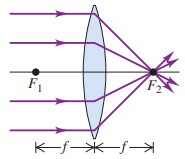
\includegraphics[width=0.65\linewidth]{LenteConvergente1.jpg}
        \captionof{figure}{\textit{Física universitaria} [Figura], por Sears, Zemansky, 2018: Lente convergente}
        \label{rayos LC}
    \end{Figure}

    Los lentes divergentes se caracterizan por ser más gruesos en sus bordes que en su centro. Al ser atravesados por un haz de rayos paralelos al eje óptico, emergen de la lente como si divergieran de $F_{2}$ (Fig. \ref{Rayos LD}). Si los rayos incidentes parecieran converger al punto focal $F_{1}$, al refractarse se dirigirán paralelamente al eje óptico.

    \begin{Figure}
        \centering
        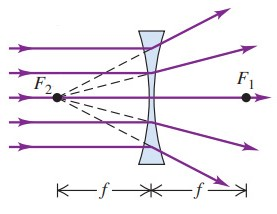
\includegraphics[width=0.75\linewidth]{RayosLD.jpg}
        \captionof{figure}{\textit{Física universitaria} [Figura], por Sears, Zemansky, 2018: Lente divergente}
        \label{Rayos LD}
    \end{Figure}

    \subsection*{Formación de imágenes en una lente convergente}

        Las imágenes formadas cuando la distancia objeto es mayor que la distancia focal son reales, siendo posible recogerlas en una pantalla. Al colocar un objeto en uno de los lados del lente, su imagen se formará  del lado opuesto a este, como se muestra en la figura \ref{Diag rayos LC}a, la imagen es invertida y más pequeña. Si la distancia objeto es menor que la distancia focal, la imagen que se forma es virtual, siendo imposible recogerla con una pantalla (la imagen se construye a partir de la prolongación de los rayos refractados), como se muestra en la figura \ref{Diag rayos LC}b, la imagen es derecha y más grande.

        % Diagrama de rayos LC
        \begin{Figure}
            \centering
            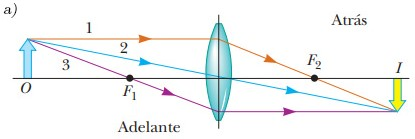
\includegraphics[width=1\linewidth]{DiagramaRayosLC1.jpg}
        \end{Figure}

        \begin{Figure}
            \centering
            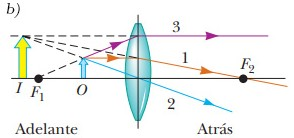
\includegraphics[width=0.7\linewidth]{DiagramaRayosLC2.jpg}
            \captionof{figure}{\textit{Physics for Scientists and Engineers} [Figura], por Serway, Jerwett, 2004: Diagrama de rayos, lente convergente}
            \label{Diag rayos LC}
        \end{Figure}

       En la figura se muestran rayos que divergen de un punto del objeto. Para simplificar el diagrama, se trazan 3 rayos principales:

        \begin{enumerate}
            \item Rayo paralelo al eje, se refracta y pasa por el punto focal $F_{2}$.
            \item Rayo que pasa por el centro de la lente, la desviación no es apreciable por lo que sigue una línea recta.
            \item Rayo que pasa por el punto focal $F_{1}$ y emerge paralelo al eje.
        \end{enumerate}

    \subsection*{Formación de imágenes en una lente divergente}

        La distancia focal en las lentes divergentes es siempre negativa, es decir, un objeto real siempre formará imágenes virtuales. Esta imagen es siempre de menor tamaño y próxima al lente, como se muestra en la figura \ref{f: rayos LD}. En caso de tratarse de un objeto virtual, la imagen formada es real.

        % Diagrama de rayos LD
        \begin{Figure}
            \centering
            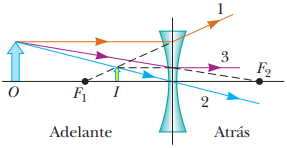
\includegraphics[width=0.9\linewidth]{DiagRayosLD.png}
            \captionof{figure}{\textit{Physics for Scientists and Engineers} [Figura], por Serway, Jerwett, 2004: Diagrama de rayos, lente divergente}
            \label{f: rayos LD}
        \end{Figure}

        Al igual que la figura \ref{Diag rayos LC}, se trazan 3 rayos:

        \begin{enumerate}
            \item Rayo paralelo al eje que al refractarse por la lente parece provenir del punto focal $F_{1}$, se aleja de $F_{2}$.
            \item Rayo que pasa por el centro de la lente, la desviación no es apreciable por lo que sigue una línea recta.
            \item Rayo con dirección de $F_{2}$ que al refractarse emerge de la lente paralelo al eje.
        \end{enumerate}

    \subsection*{Aberraciones}

        En una situación ideal, todos los rayos que inciden en la lente convergen en el mismo punto, sin embargo en la realidad, los rayos paraxiales y los rayos periféricos convergen en distintos puntos. Este fenómeno recibe el nombre de \emph{aberración de esfericidad}, ilustrada en la figura \ref{f:abesf}. El punto de convergencia de los rayos paraxiales se encuentra más lejos que el de los rayos periféricos, que convergen más cerca de la lente. Esto genera que la imágen obtenida no tenga nitidez en ningun punto y no se cumple el modelo. Es posible reducir la aberración implementando un diafragma, es decir, un dispositivo que bloquea el camino óptico de los rayos no deseados.

        %aberraciones
        \begin{Figure}
            \centering
            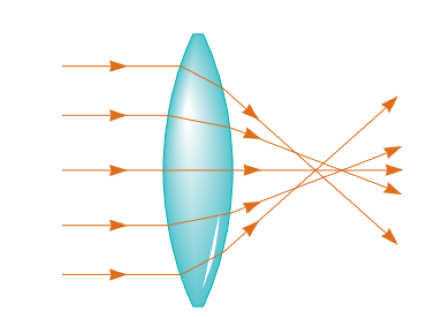
\includegraphics[width=0.7\linewidth]{AberracionEsferica.png}
            \captionof{figure}{\textit{Physics for Scientists and Engineers} [Figura], por Serway, Jerwett, 2004: Aberración de esfericidad}
            \label{f:abesf}
        \end{Figure}

        Otro tipo de aberración que se presenta en los lentes es la \emph{aberración cromática}, que se debe a la variación del indice de refracción con respecto de la longitud de onda. Al pasar luz blanca a través de una lente, se refracta de manera que los rayos azules convergen más cerca del lente y los rojos más lejos, mientras que los rayos verdes convergen en un punto intermedio, como se muestra en la figura \ref{f: abcro}.

        \begin{Figure}
            \centering
            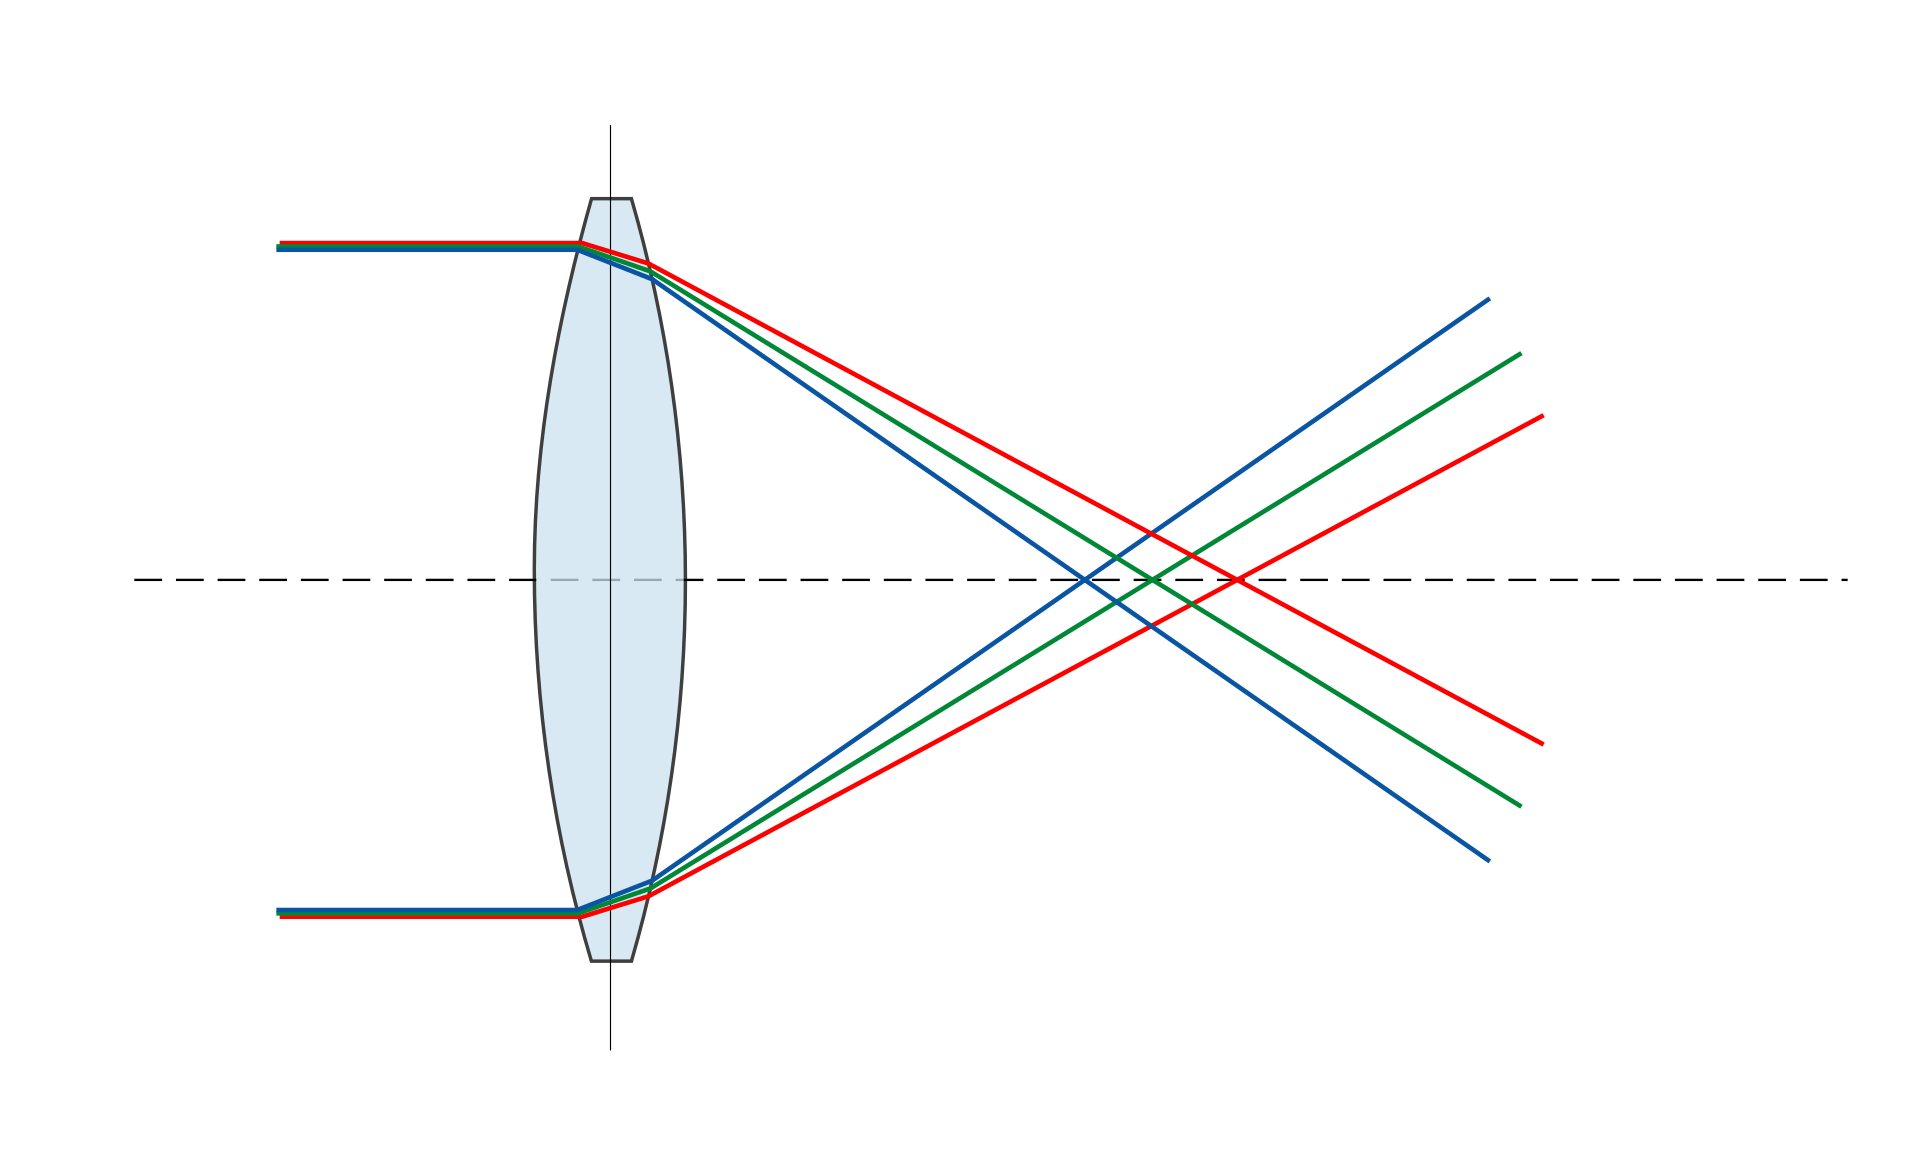
\includegraphics[width=0.9\linewidth]{AberracionCromatica.png}
            \captionof{figure}{\textit{Illustration of chromatic abberation with a convergent lens} [Figura], por Bajart, 2010: Aberración cromática. CC BY SA 3.0}
            \label{f: abcro}
        \end{Figure}
        
    \subsection*{Telescopios de refracción}

        Una de las aplicaciones de los sistemas compuestos de lentes son los telescopios de refracción, el cual consta de un sistema de dos lentes, una lente objetivo y una lente ocular. La distancia entre objetivo y ocular, que es la longitud del telescopio, es la suma de las distancias focales.

        \begin{equation} \label{eq:disTel}
            L_{T}=f_{ob}+f_{oc}
        \end{equation}

        \begin{Figure}
            \centering
            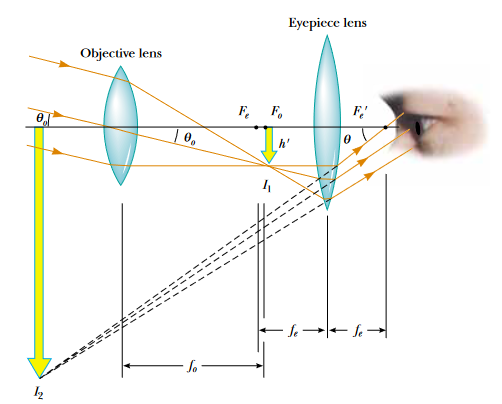
\includegraphics[width=0.8\linewidth]{telescopio.png}
            \captionof{figure}{\textit{Physics for Scientists and Engineers} [Figura], por Serway, Jerwett, 2004: Diagrama de rayos, telescopio de Kepler}
            \label{fig: diagTelescopio}
        \end{Figure}

        Los telescopios nos permiten ver objetos de gran tamaño que se encuentran a grandes distancias. Consideraremos infinita la distancia objeto, de manera que los rayos inciden todos paralelos y su imagen estará formada en el foco. 

        Podemos definir el aumento angular de un telescopio como la razón entre los ángulos $\theta_{0}$ y $\theta$, donde $\theta_{0}$ es el ángulo que se forma entre el objeto y la lente objetivo, y $\theta$ es el ángulo que se forma entre la imagen final y el ojo del observador. Matemáticamente podemos trabajar con esta razón para llegar a la ecuación:

        \begin{equation} \label{eq: aumentoTel}
            m=\frac{\theta}{\theta_{0}}=-\frac{f_{ob}}{f_{oc}}
        \end{equation}

        El signo negativo se debe a que la imagen final está invertida.

        El telescopio de Kepler consta de dos lentes convergentes, de manera que la imagen real invertida formada por la lente objetivo se encuentra próxima al foco de la lente ocular, donde para esta actúa como objeto real formando una imagen virtual derecha respecto a la primera y de mayor tamaño, lo que resulta en una imagen final invertida y de mayor tamaño que el objeto.

        El telescopio de Galileo consta de una lente convergente (objetivo) y una lente divergente (ocular), donde el comportamiento de la lente objetivo es el mismo al telescopio de Kepler, sin embargo la imagen real invertida actúa ahora como objeto virtual para la lente ocular, que genera una imagen virtual invertida con respecto a la real, y de menor tamaño, que resulta en una imagen final derecha y de menor tamaño que el objeto.

\section*{Método experimental}

    \subsection*{Lente convergente}

        Con el objetivo de comprobar experimentalmente la relación entre la distancia imagen y la distancia objeto para una lente convergente (Ecuación \ref{eq:1/i+1/o}), hemos diseñado un sistema experimental a partir del equipo \emph{PASCO Basic Optics System} (Fig. \ref{PASCOconv}) con el que poder determinar si el modelo es aplicable.

        El sistema experimental consta de un riel milimetrado en el que colocamos una fuente luminosa, una lente convergente, y una pantalla como se observa en la figura \ref{PASCOconv}. La distancia objeto (o) es la distancia entre la fuente y la lente, que medimos utilizando el cursor del soporte de la lente, mientras que la distancia imagen (i) será la distancia entre la lente y la pantalla.

        Al momento de usar el sistema experimental, lo que se hará es mover el lente, y ver dónde está la imagen real después del cambio.

        % Diagrama lente convergente
        \begin{Figure}
            \centering
            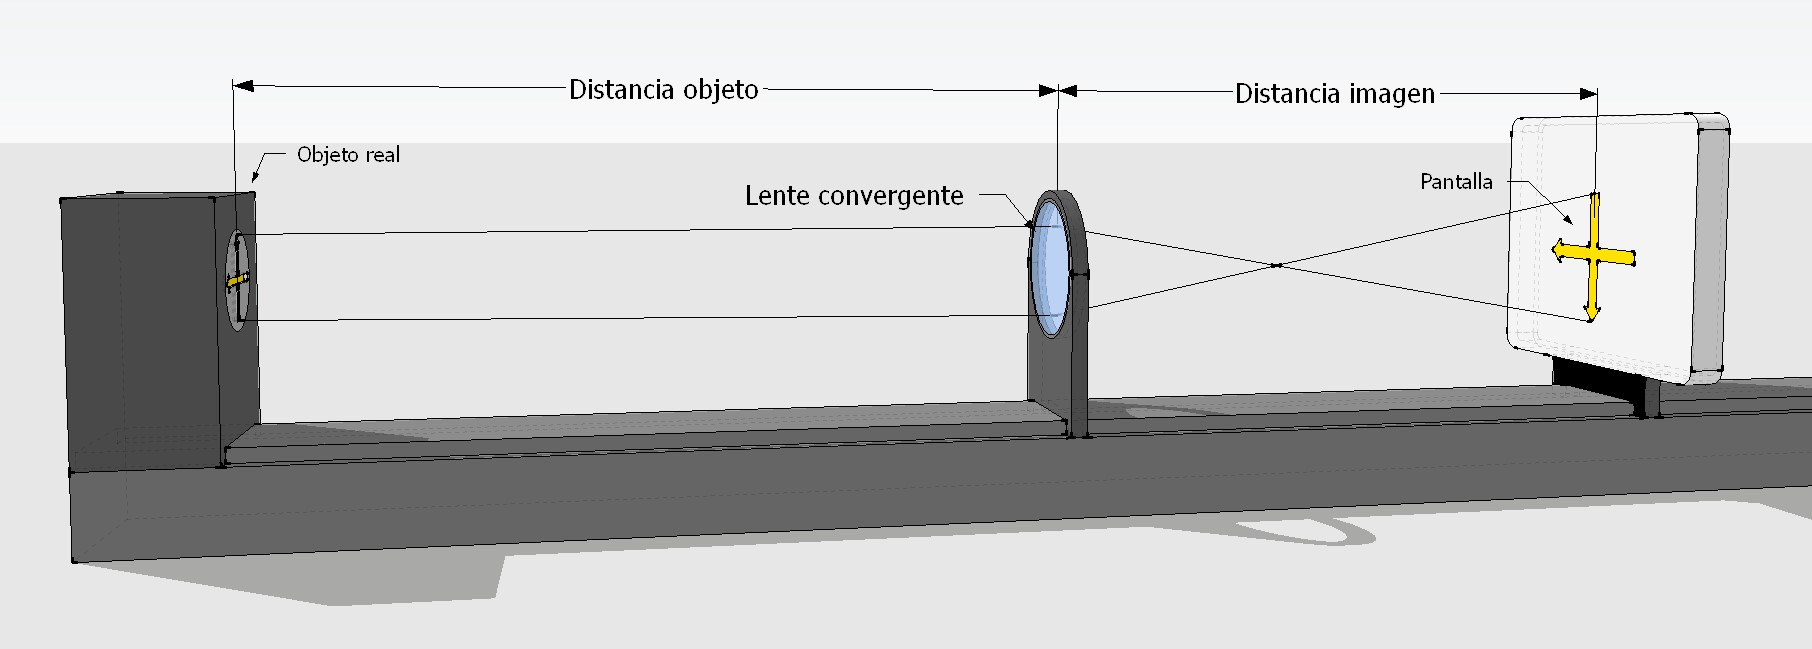
\includegraphics[width=1\linewidth]{LenteConvergente.jpg}
            \captionof{figure}{Diagrama sistema lente convergente}
            \label{PASCOconv}
        \end{Figure}

    \subsection*{Lente divergente}

        El sistema experimental utilizado para medir las distancias objeto e imagen de una lente divergente fue creado a partir del mismo equipo utilizado para la lente convergente, el mismo hace uso de una lente convergente para conseguir rayos que incidan de forma convergente hacia la lente deseada. El diagrama se encuentra en la figura \ref{fig:Diagramaconvex}, como se observa los rayos refractados por la lente divergente logran formar una imagen real cuya distancia es medible experimentalmente.

        % Diagrama Lente divergente
        \begin{Figure}
            \centering
            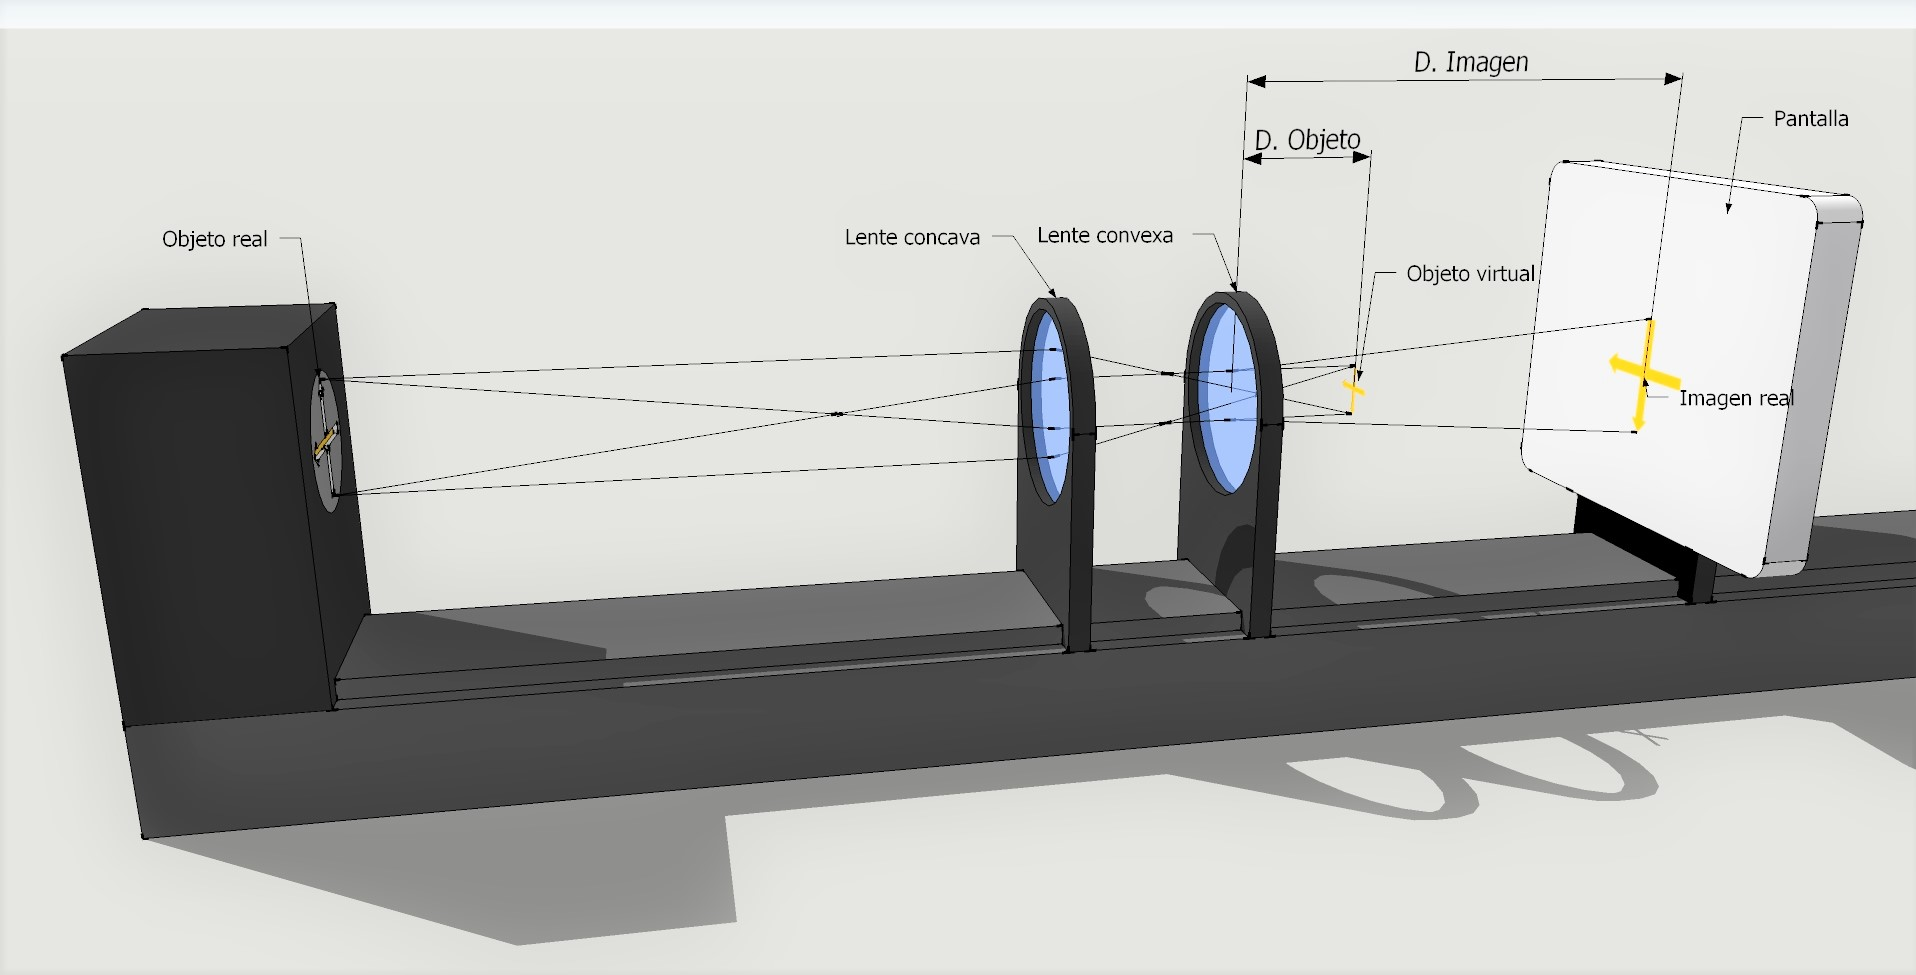
\includegraphics[width=1\linewidth]{DLCX}
            \captionof{figure}{Diagrama sistema lente divergente}
            \label{fig:Diagramaconvex}
        \end{Figure}

        En la figura también se aprecia las distancias imagen (\emph{i}) y objeto (\emph{o}) que deseamos medir. Comenzamos ubicando la lente convergente y midiendo la posición de la imagen formada, la cual utilizaremos como \emph{objeto virtual} para la lente divergente. A esta ultima la colocamos entre la imagen y la lente convergente, luego comenzamos a moverla hasta que observemos que se forma la imagen en la pantalla. Una vez ubicada la posición donde la imagen es nítida, medimos la distancia de la pantalla a la lente divergente. Las mediciones se realizan de manera directa utilizando la escala horizontal ubicada sobre el riel que se observa en la figura \ref{fig:Diagramaconvex}. A la hora de ubicar la posición de las imágenes reales de las lentes se ha de considerar un intervalo de longitud en el cual la imagen es nítida y no un único punto.

        Para los siguientes puntos simplemente desplazamos la lente divergente (sin sobrepasar al objeto virtual), encontrando las imágenes en la pantalla, y midiendo las distancias.

    \subsection*{Telescopios de refracción}

        El sistema experimental utilizado para analizar el funcionamiento de los telescopios de Kepler y de Galileo consta de un riel milimetrado, una lente convergente de $f=500$ $mm$ que actúa de lente objetivo, otra lente convergente de $f=250$ $mm$ que actúa como lente ocular para el telescopio de Kepler, y una lente divergente de $f=-100$ $mm$, que actúa como ocular para el telescopio de Galileo.

        \begin{Figure}
            \centering
            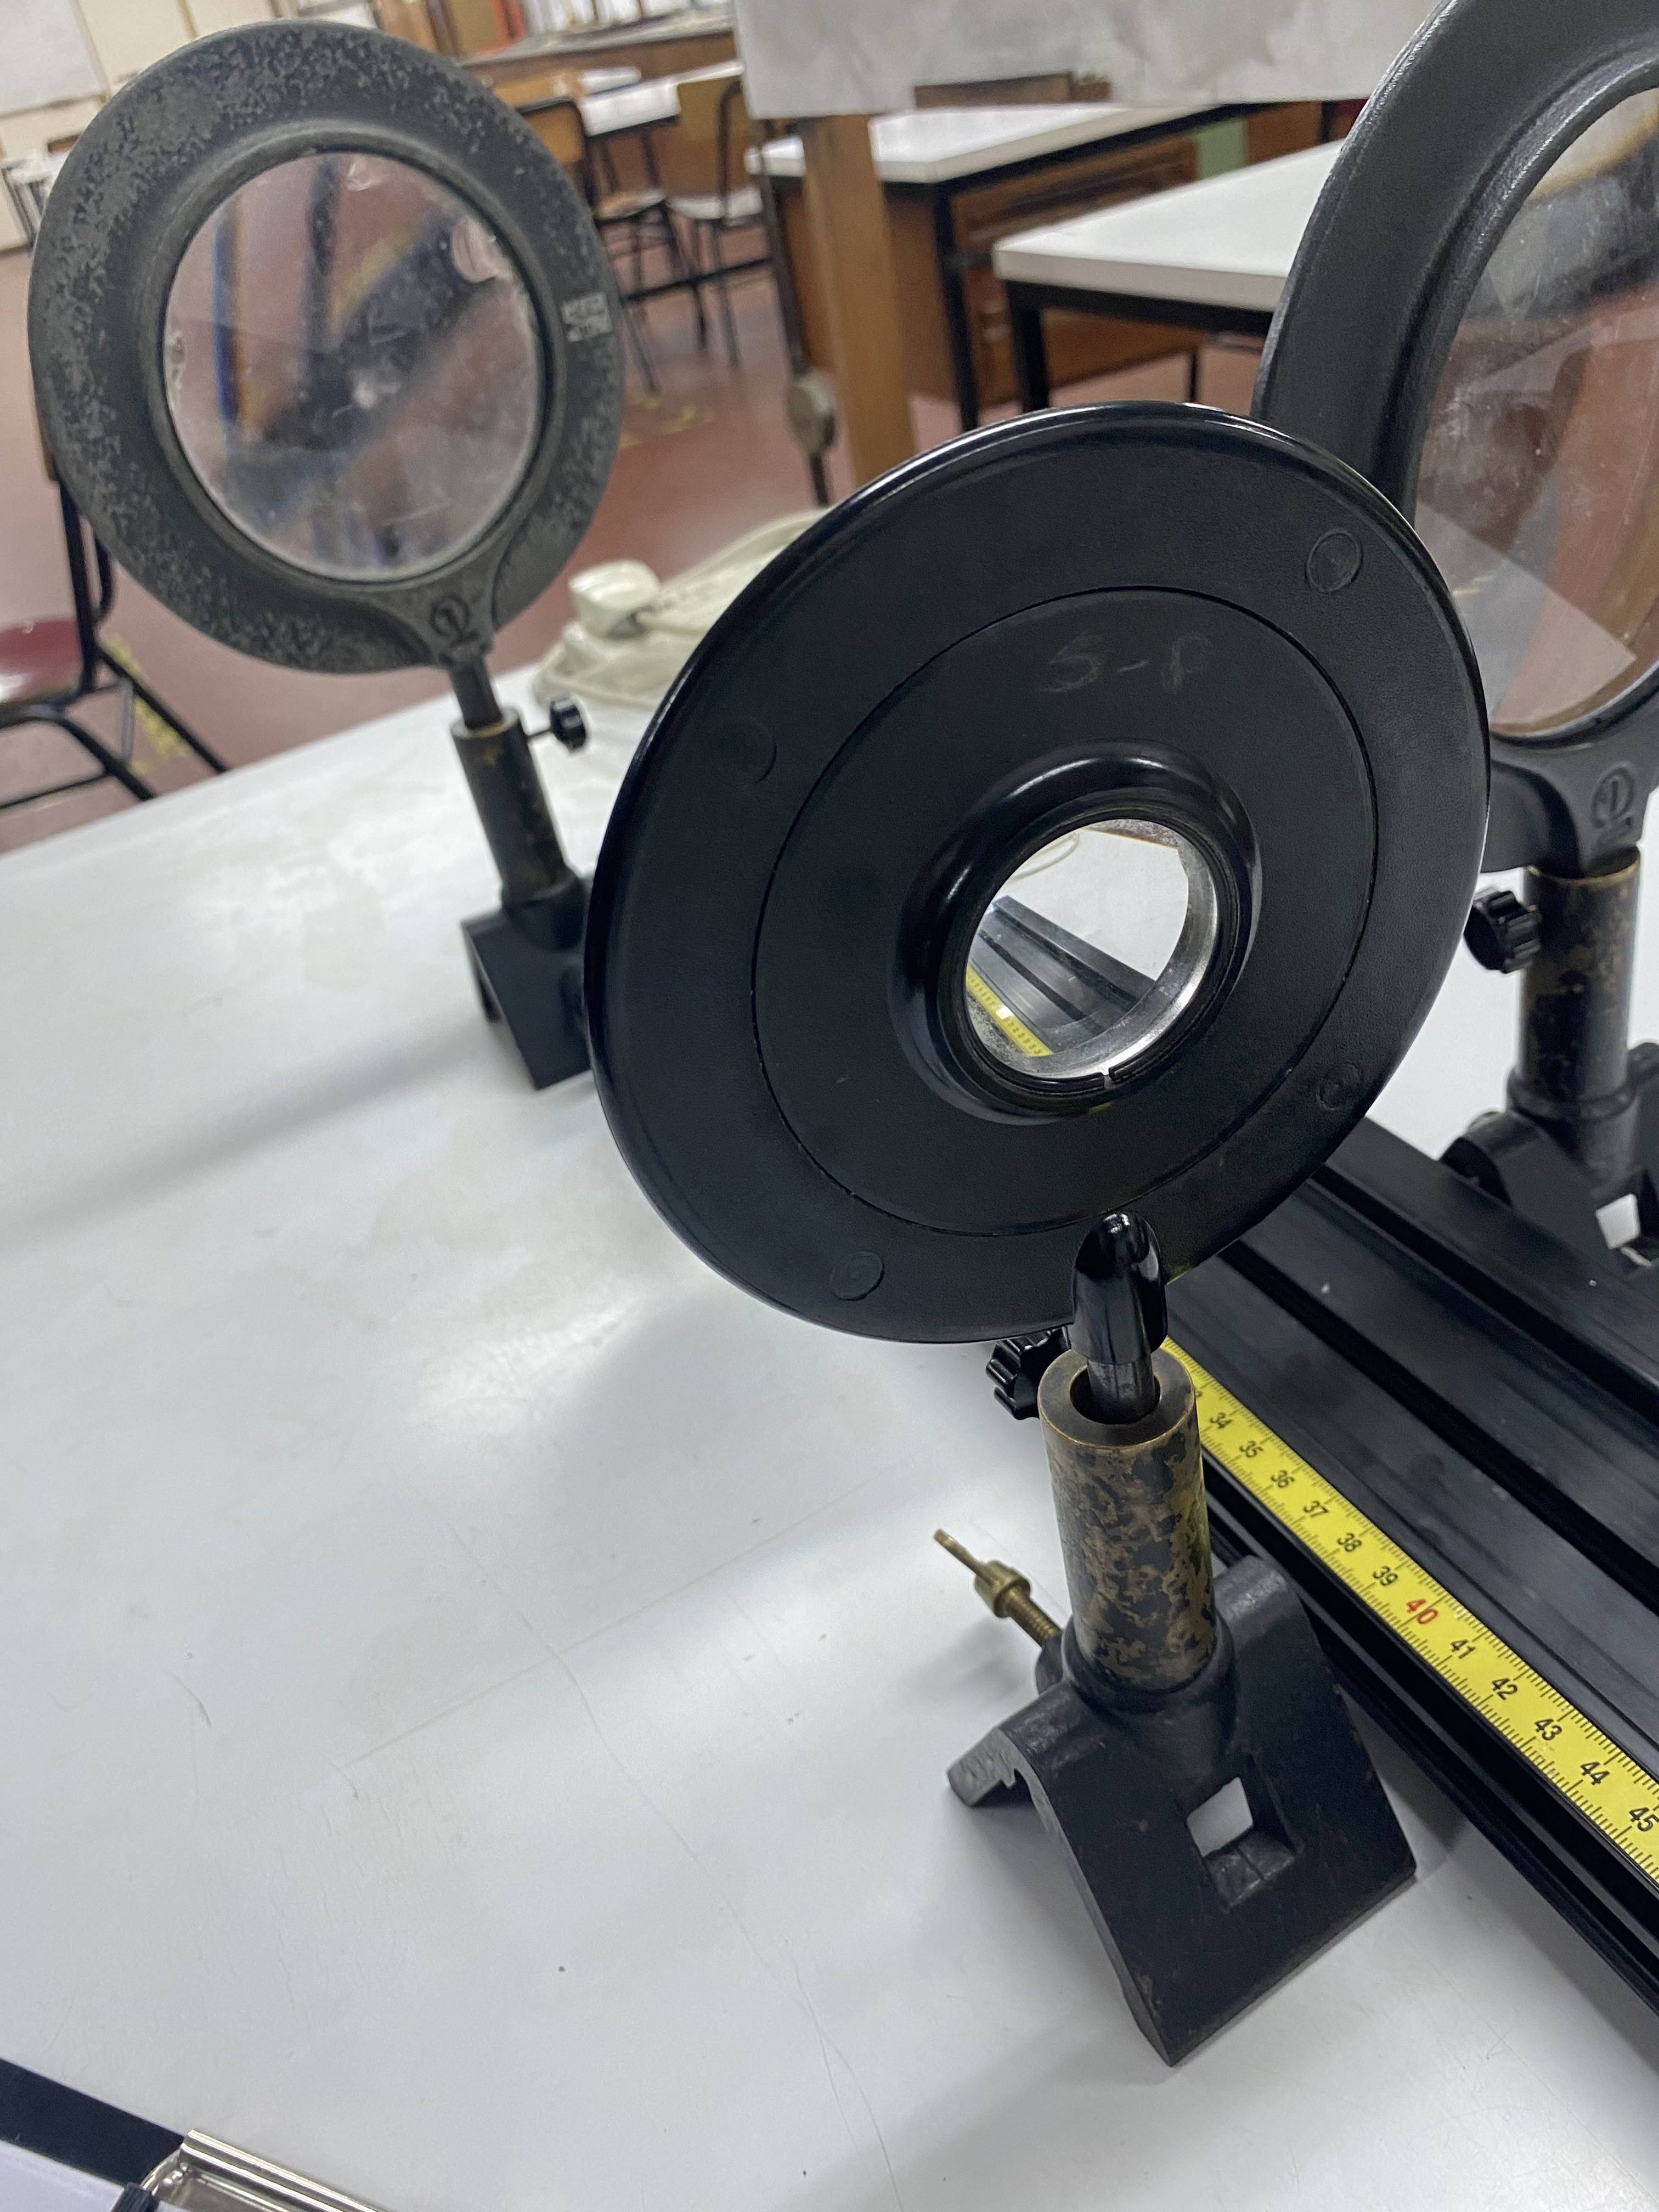
\includegraphics[width=0.55\linewidth]{SistTelRR.jpg}
            \captionof{figure}{Sistema experimental telescopio de Kepler}
            \label{f: Tel}
        \end{Figure}

        La distancia entre las lentes se consigue con la ecuación (\ref{eq:disTel}).

\section*{Datos y resultados}

    \subsection*{Lente convergente}

        Las mediciones para la lente convergente son las mostradas en las tablas \ref{i vs o lc} y \ref{1/i vs 1/o lc}, donde como previamente mencionado en el desarrollo experimental, se fue variando la posición de la lente convergente (y por lo tanto la distancia objeto), y se determinó dónde está la imagen. Si el modelo es aplicable, deberíamos de poder ver una relación lineal entre las inversas de estos valores de la forma:

        \begin{equation*}
            \frac{1}{i} = \frac{1}{f} - \frac{1}{o}
        \end{equation*}

        Por lo que la pendiente de la gráfica debe ser -1 dentro del error, y la ordenada será la inversa de la distancia focal de la lente.

        El error de la distancia objeto es el error de apreciación a la hora de medir la posición de la fuente luminosa y la lente convergente. El error de la distancia imagen es la suma de los errores de apreciación de la fuente y la pantalla, y el error de definición que se tomó como la mitad del intervalo de nitidez de la imagen que para reducirlo, seleccionamos una pequeña sección reconocible del objeto para revisar su nitidez.

        % Tabla i vs o lente convergente
        \begin{Figure}
            \centering

            \begin{tabular}{cc}
                \toprule
                \textit{\textbf{o $\pm$ $\Delta$o [mm]}} & \textit{\textbf{i $\pm$ $\Delta$i [mm]}}\\
                \midrule
                $200 \pm 2$ & $193 \pm 8$ \\ 
                $300 \pm 2$ & $148 \pm 5$ \\ 
                $400 \pm 2$ & $133 \pm 4$ \\ 
                $500 \pm 2$ & $125 \pm 4$ \\ 
                $600 \pm 2$ & $120 \pm 4$ \\ 
                $700 \pm 2$ & $116 \pm 4$ \\ 
                $800 \pm 2$ & $113 \pm 4$ \\    
                $900 \pm 2$ & $113 \pm 4$ \\ 
                $1000 \pm 2$ & $112 \pm 4$ \\ 
                \bottomrule
            \end{tabular}

            \captionof{table}{o e i para lente convergente}
            \label{i vs o lc}
        \end{Figure}

        % Tabla 1/i vs 1/o lente convergente
        \begin{Figure}
            \centering

            \begin{tabular}{cc}
                \toprule
                \textit{\textbf{$\frac{1}{o}$ $\pm$ $\Delta{\frac{1}{o}}$ [$mm^{-1}$]}} & \textit{\textbf{$\frac{1}{i}$ $\pm$ $\Delta{\frac{1}{i}}$ [$mm^{-1}$]}}\\
                \midrule
                $0,00500 \pm 0,00005$ & $0,0052 \pm 0,0002$ \\ 
                $0,00333 \pm 0,00002$ & $0,0068 \pm 0,0002$ \\ 
                $0,00250 \pm 0,00001$ & $0,0075 \pm 0,0002$ \\ 
                $0,002000 \pm 0,000008$ & $0,0080 \pm 0,0003$ \\ 
                $0,001667 \pm 0,000006$ & $0,0083 \pm 0,0003$ \\ 
                $0,001429 \pm 0,000004$ & $0,0086 \pm 0,0003$ \\ 
                $0,001250 \pm 0,000003$ & $0,0088 \pm 0,0003$ \\ 
                $0,001111 \pm 0,000002$ & $0,0088 \pm 0,0003$ \\ 
                $0,001000 \pm 0,000002$ & $0,0089 \pm 0,0003$ \\
                \bottomrule
            \end{tabular}

            \captionof{table}{$o^{-1}$ e $i^{-1}$ para lente convergente}
            \label{1/i vs 1/o lc}
        \end{Figure}

        \begin{Figure}
            \centering
            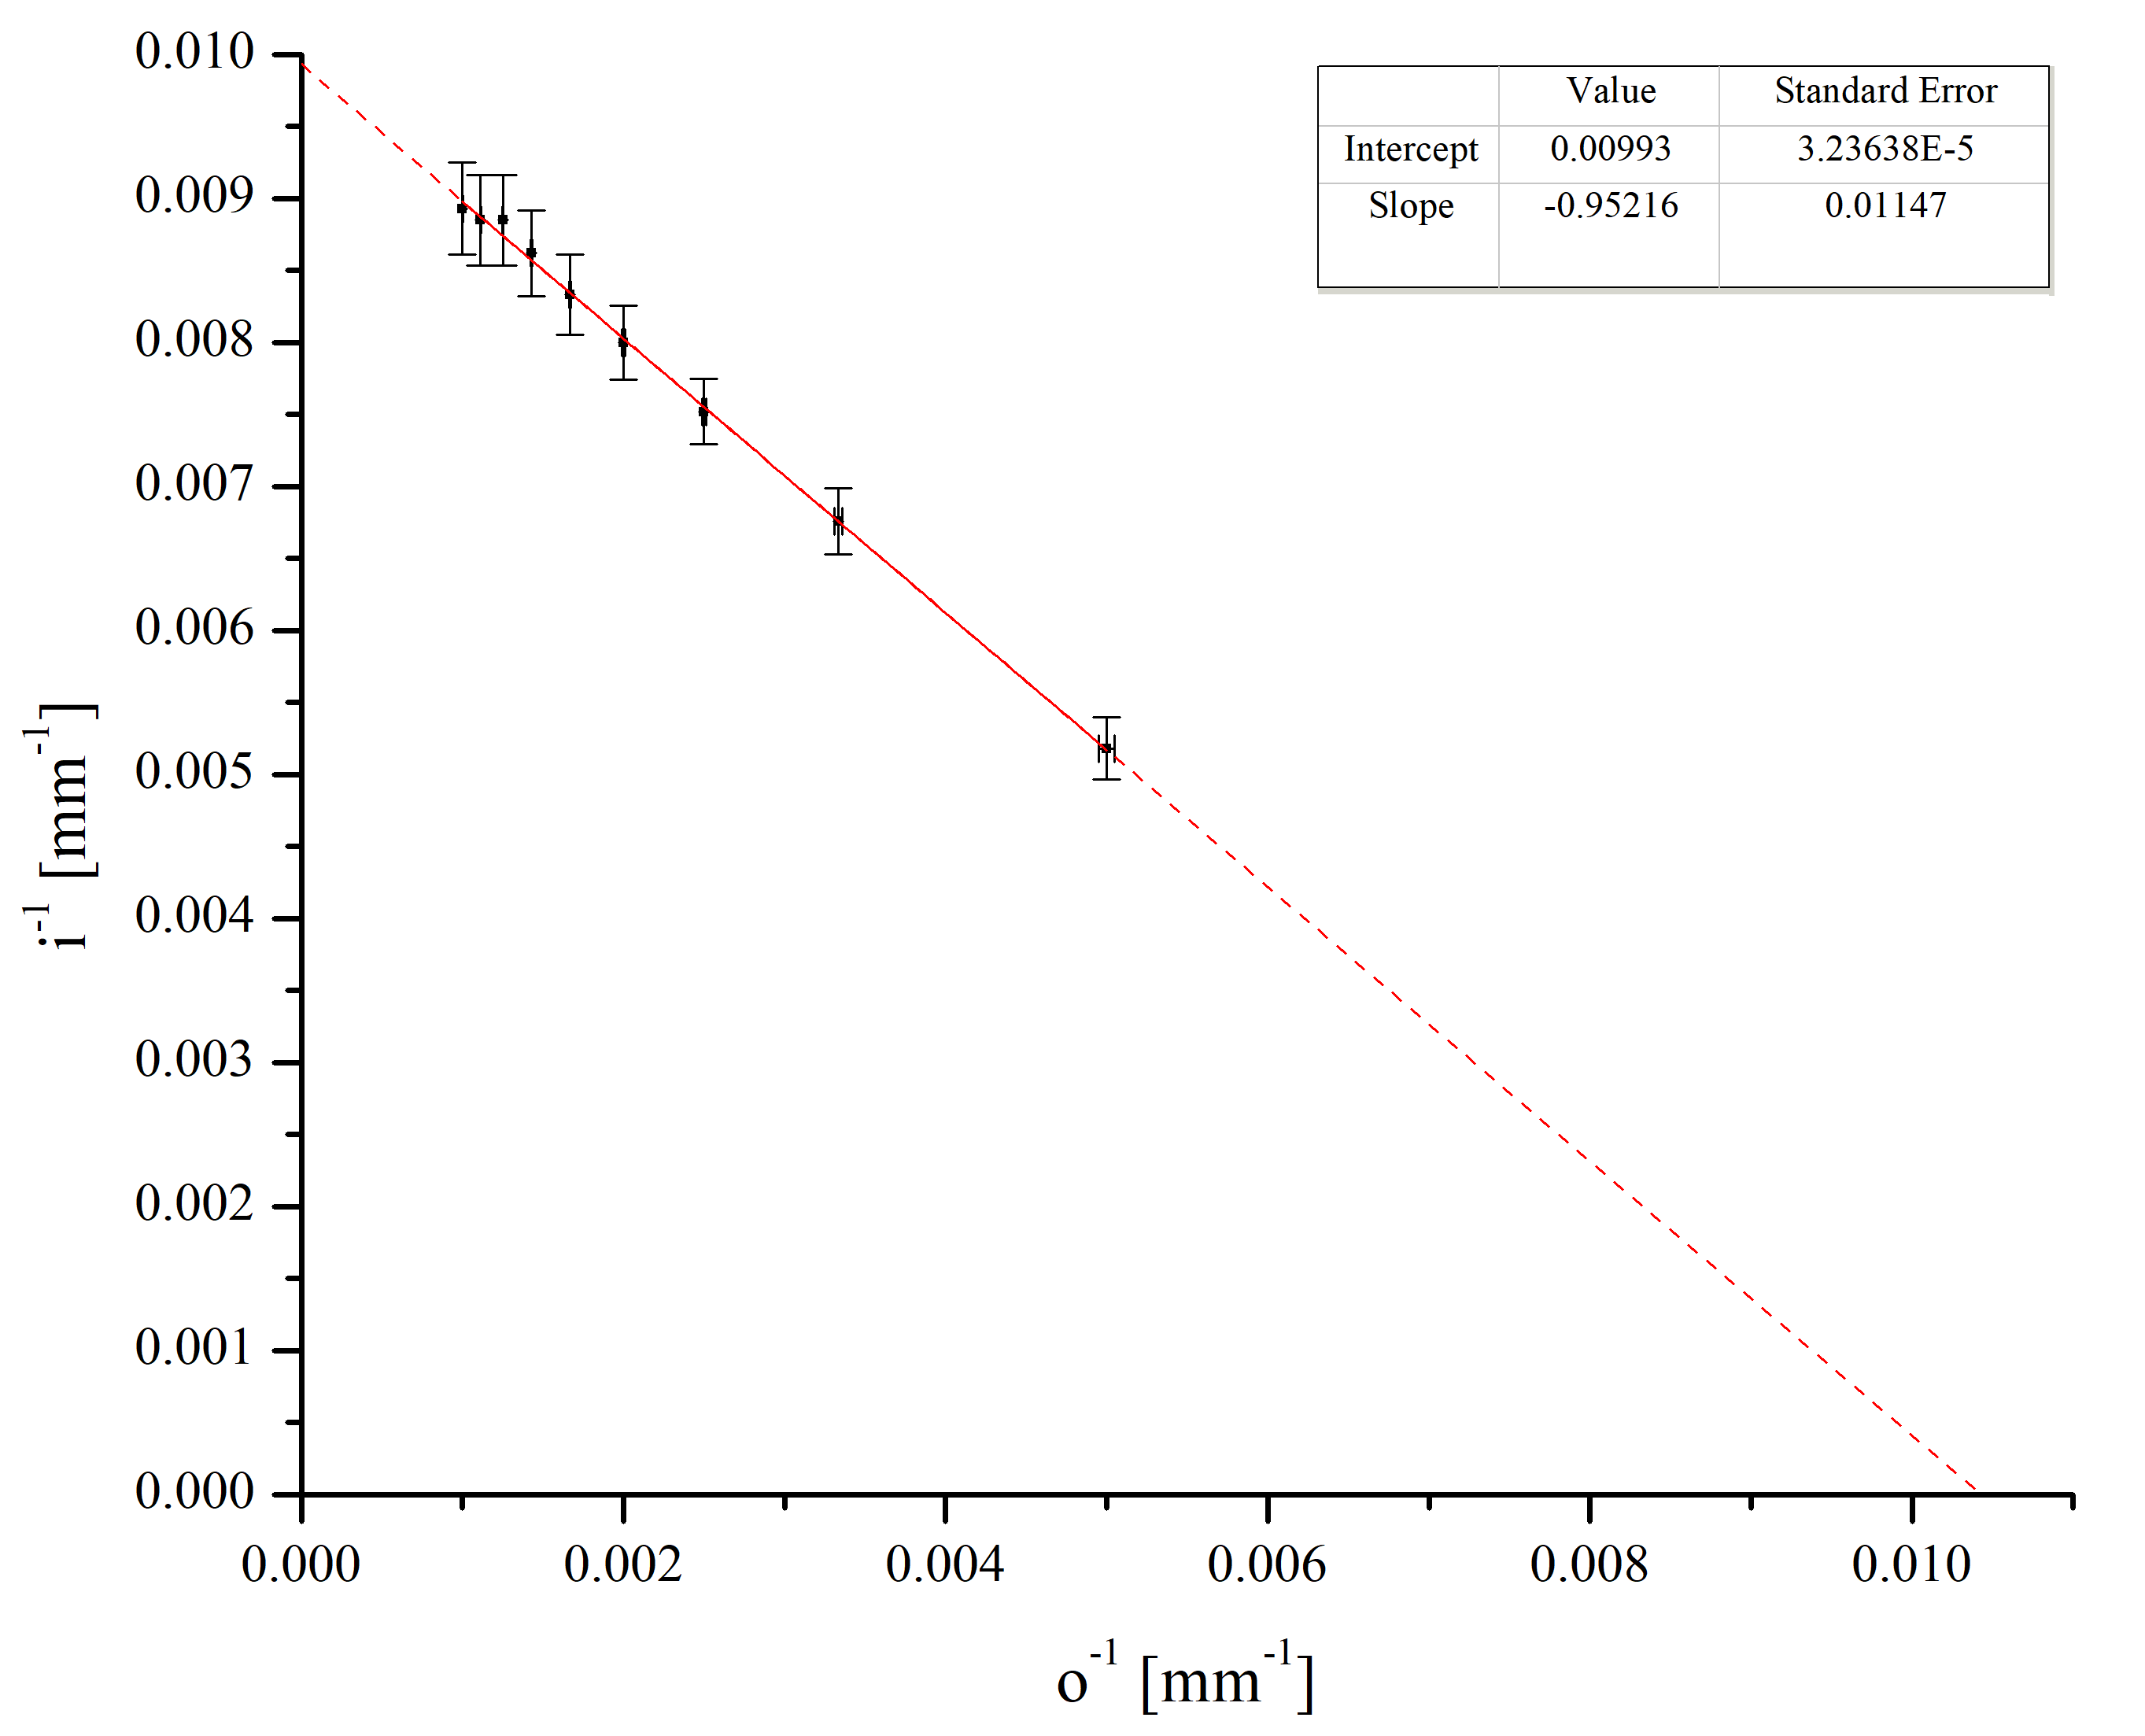
\includegraphics[width=0.95\linewidth]{GraficaLC.png}
            \captionof{figure}{$i^{-1}$ vs $o^{-1}$ para la lente convergente}
            \label{grafica lc}
        \end{Figure}

        Los parámetros de la recta calculados con el método de cuadrados mínimos, y con el error siendo la suma de dicho método y del método gráfico son:

        Pendiente: $(-0.9 \pm 0.1)$

        Ordenada: $(9.9$ $\pm$ $0.3)$ . $10^{-3}$ $mm^{-1}$

        Como el valor de la pendiente está dentro de lo esperado por el modelo, y la recta se ajusta a los datos, podemos calcular la distancia focal de la lente como $f = (101 \pm 3)$ $mm$, y la distancia focal de la lente dada por el fabricante es $f = (100 \pm 1)$ $mm$.

    \subsection*{Lente divergente}

        Los resultados de las mediciones del sistema de la lente divergente se encuentran colocados en las tablas \ref{tab:Datosdivnor} y \ref{tab:Datosdiverinv}, todas las mediciones fueron acotadas con 1 mm de apreciación, y para aquellas relacionadas con las imágenes de las lentes se les agrego un error de definición el cual consiste en la mitad del intervalo de nitidez mencionado anteriormente en el desarrollo experimental. Para reducir este intervalo, decidimos considerar una pequeña sección del objeto a la hora de revisar su nitidez. Los valores de la tabla \ref{tab:Datosdiverinv} se encuentran graficados en la figura \ref{fig:Lentediv}.

        En este caso se graficó $o^{-1}$ vs $i^{-1}$ para poder realizar el ajuste por cuadrados mínimos, y sumando las incertidumbres experimentales y analíticas obtenemos el error.

        %NORMALES LENTE DIVERGENTE
        \begin{Figure}
            \centering

            \begin{tabular}{cc}
                \toprule
                \multicolumn{1}{c}{\textit{\textbf{o} [mm]}} & \textit{\textbf{i} [mm]} \\
                \midrule
                $(-123 \pm 5)$ & $(73 \pm 3)\times10 $\\
                $(-113 \pm 5)$ & $(48 \pm 2)\times10$ \\
                $(-103 \pm 5)$ & $(34 \pm 1)\times10$ \\
                $(-93 \pm 5)$ & $(251 \pm 6)$ \\
                $(-83 \pm 5)$& $(192 \pm 7)$ \\
                $(-73 \pm 5)$ & $(136 \pm 4)$ \\
                \bottomrule
            \end{tabular}

            \captionof{table}{o e i para lente divergente}
            \label{tab:Datosdivnor}
        \end{Figure} 

        %INVERSOS LENTE DIVERGENTE
        \begin{Figure}
            \centering

            \begin{tabular}{cc}
                \toprule
                \textit{\textbf{1/o [$mm^{-1}$]}} & \textit{\textbf{1/i [$mm^{-1}$]}} \\
                \midrule
                $(-0.0082 \pm 0.0003)$ & $(0.00138 \pm 0.00006)$ \\
                $(-0.0089 \pm 0.0004)$ & $(0.00208 \pm 0.00009)$ \\
                $(-0.0097 \pm 0.0005)$ & $(0.00293 \pm 0.00009)$ \\
                $(-0.0108 \pm 0.0006)$ & $(0.00399 \pm 0.00009)$ \\
                $(-0.0121 \pm 0.0007)$ & $(0.0052 \pm 0.0002)$ \\
                $(-0.0137 \pm 0.0009)$ & $(0.0074 \pm 0.0002)$ \\
                \bottomrule 
            \end{tabular}
            \captionof{table}{$o^{-1}$ e $i^{-1}$ para lente divergente}
            \label{tab:Datosdiverinv}
        \end{Figure}

        \begin{Figure}
            \centering
            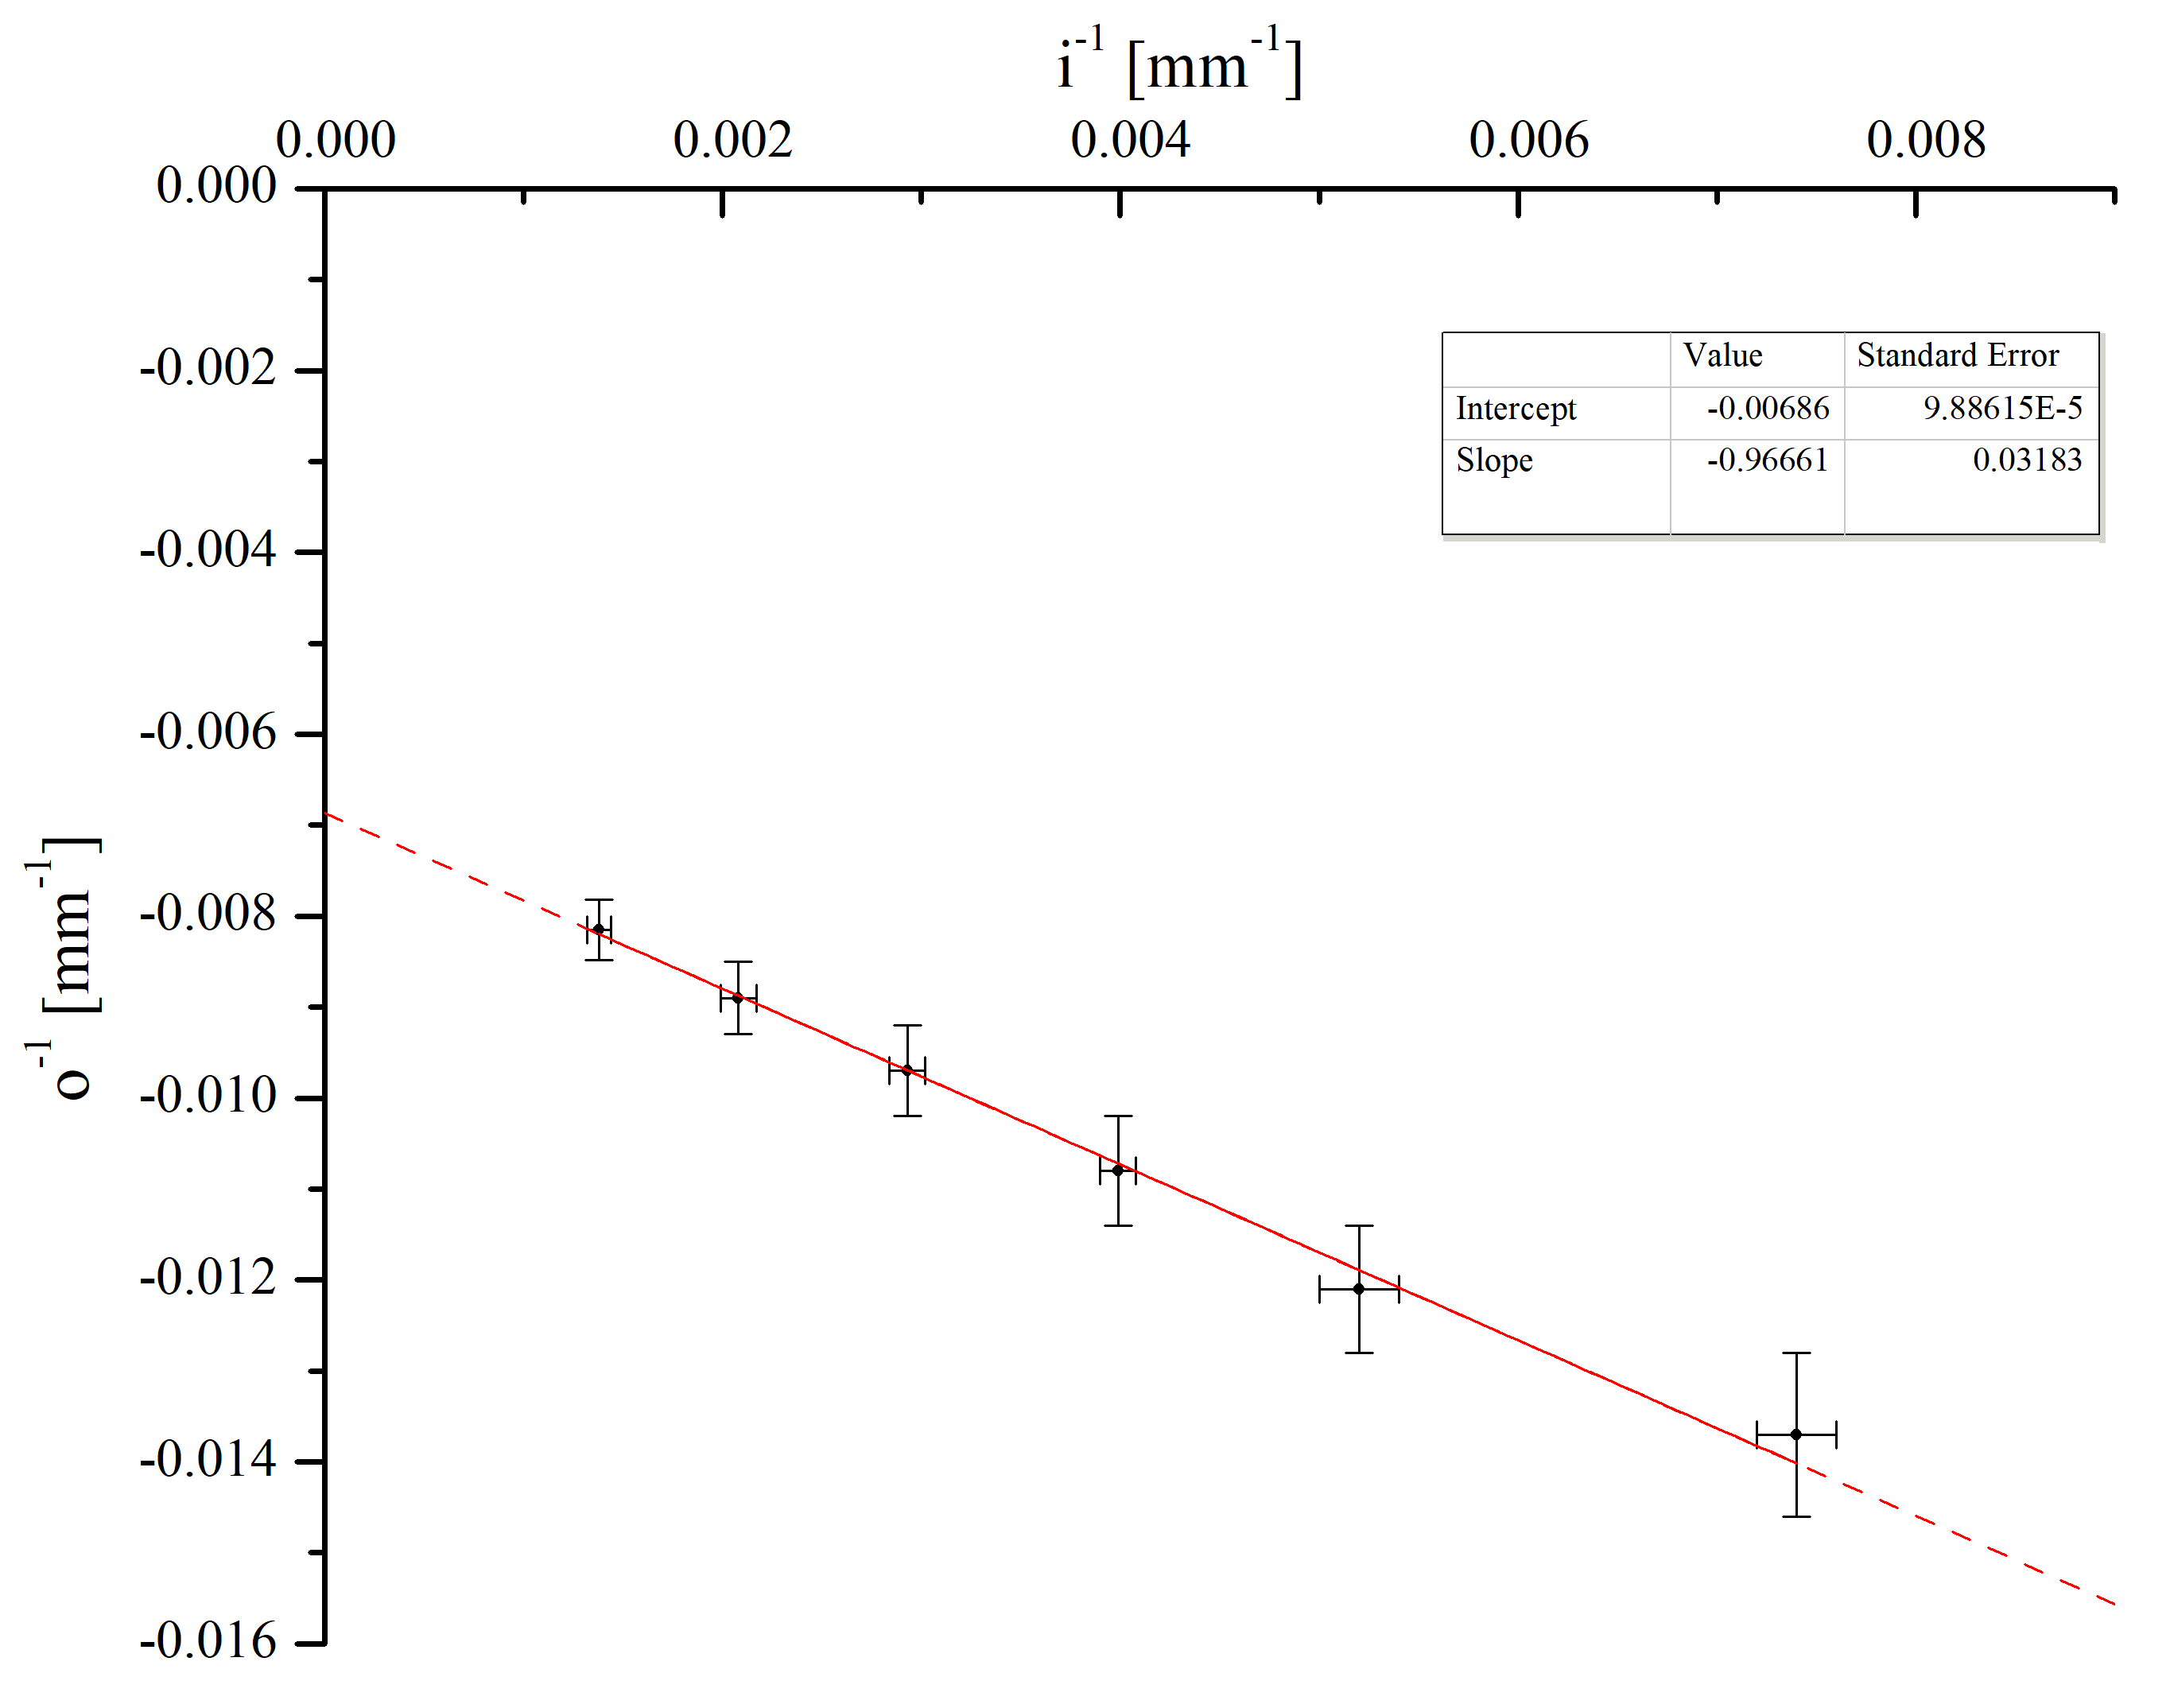
\includegraphics[width=1\linewidth]{GraficaLD.png}
            \captionof{figure}{$i^{-1}$ vs $o^{-1}$ para la lente divergente}
            \label{fig:Lentediv}
        \end{Figure}

        Los parámetros de la recta, obtenidos con método de cuadrados mínimos, con el error por método gráfico son:

        Pendiente: $A=(-0,9$ $\pm$ $0,2)$

        Ordenada: $B=(0,007$ $\pm$ $0,001)$ $mm^{-1}$

        Tanto la grafica de la figura \ref{fig:Lentediv} como la pendiente de la recta corresponden con el comportamiento que predice el modelo en la ecuación \ref{eq:1/i+1/o}, observamos entonces que podemos determinar la distancia focal como: $B=1/f$, su valor acotado es $f=(-1,4 \pm 0,2) \times 10^{2} mm$. Y la distancia focal de la lente dada por el fabricante es: $f = (-150 \pm 1) mm$.

    \subsection*{Telescopios de refracción}

        No se realizaron suficientes mediciones para comprobar la correspondencia con el modelo, sin embargo se realizó una comparación con los valores que predice el modelo, en base a las mediciones realizadas.

        Pudimos realizar dos mediciones con el telescopio de Kepler, donde se midió el tamaño angular de una regla colocada a una distancia considerable a ojo como $(10,0$ $\pm$ $0,5)$ segmentos, y se midieron viendo por la lente ocular $(5,0$ $\pm$ $0,5)$ segmentos, y $(6,5$ $\pm$ $0,5)$ segmentos, donde la variación de estas dos mediciones viene dada porque fue medido por dos personas distintas con distinto punto próximo.

        \begin{Figure}
            \centering
            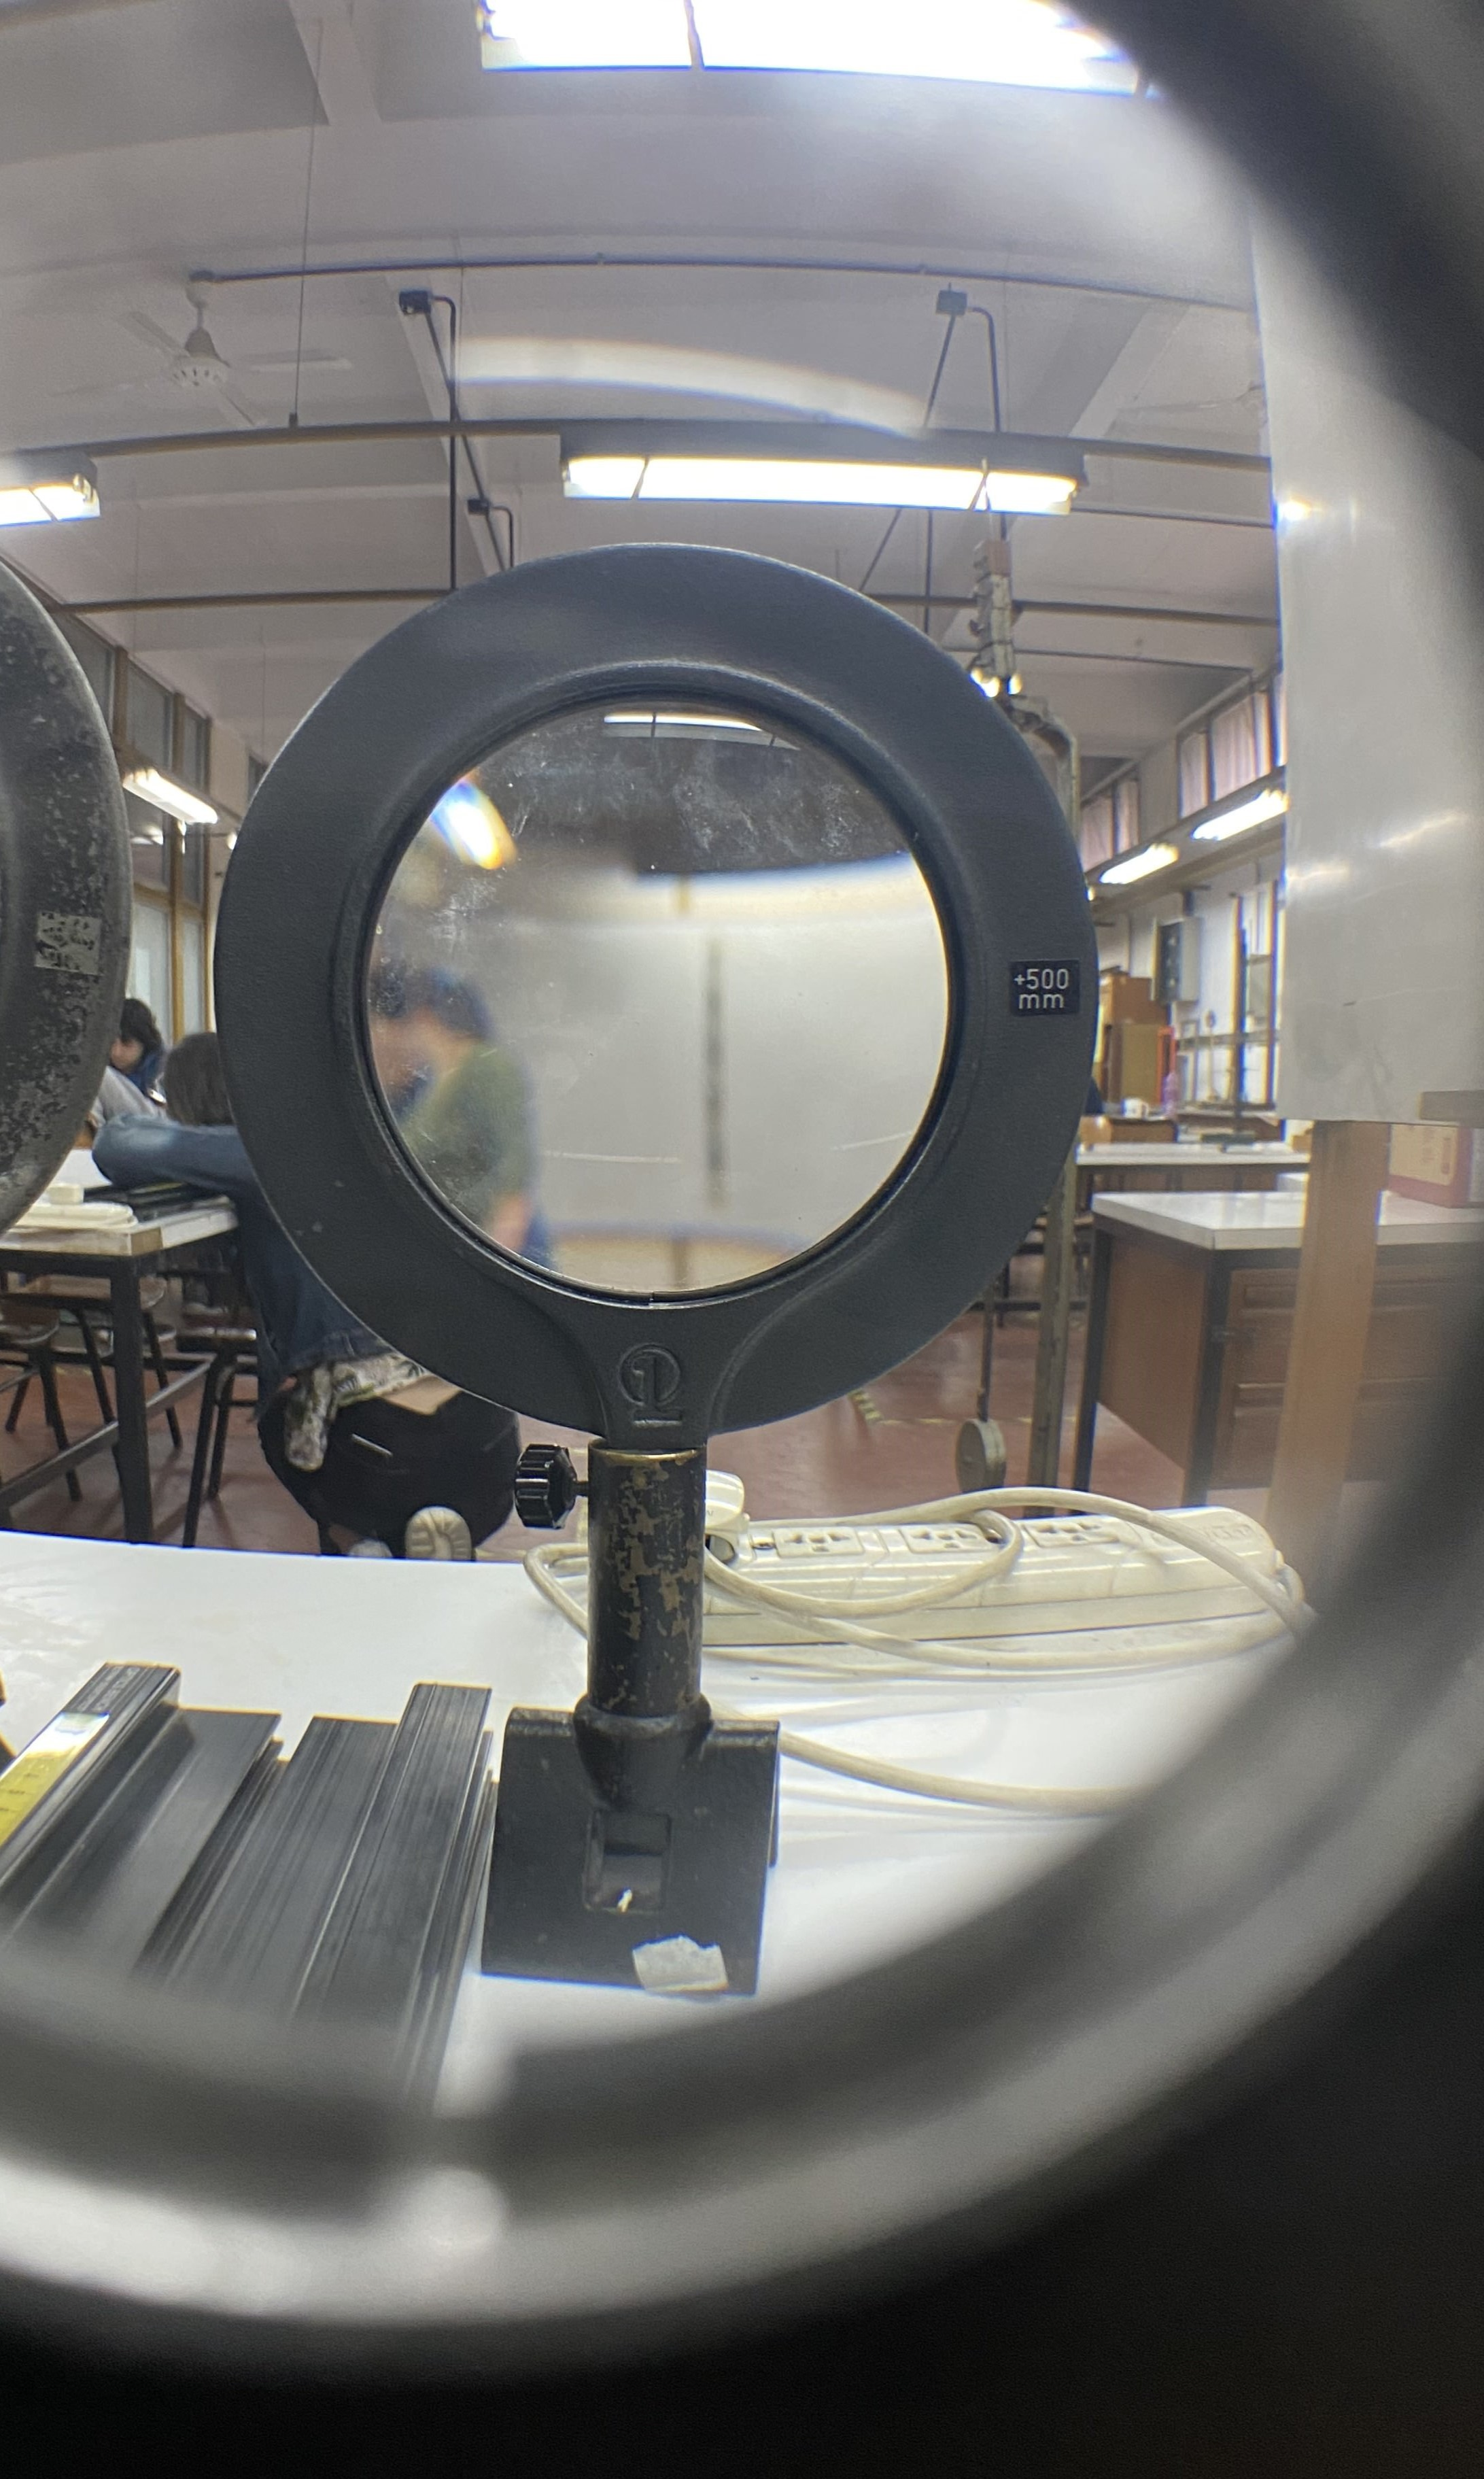
\includegraphics[width=0.5\linewidth]{MedTel.jpg}
            \captionof{figure}{Mediciones con telescopio}
            \label{f: MedTel}
        \end{Figure}

        Si calculamos el aumento del telescopio de Kepler con las mediciones obtenidas, obtenemos m = $(-2,0$ $\pm$ $0,1)$ y m = $(-1,5$ $\pm$ $0,1)$, que podemos comparar con el aumento angular teórico del telescopio, calculado usando la ecuación \ref{eq: aumentoTel}, y obtenemos m = $(-2,00$ $\pm$ $0,01)$.

    \subsection*{Control de supuestos}

        Verificamos si en nuestro diseño experimental son o no apreciables las aberraciones de esfericidad (Fig. \ref{f:abesf}) o cromáticas (Fig. \ref{f: abcro}) y controlamos los supuestos con los siguientes sistemas experimentales:

        \begin{itemize}
            \item Para las \emph{aberraciones de esfericidad} utilizamos dos diafragmas, figura \ref{f: Dparax} y figura \ref{f: Dmarg}, que interfieren el camino óptico de los rayos paraxiales y de los rayos periféricos respectivamente.
            \item Para las \emph{aberraciones cromáticas} utilizamos dos acetatos, uno de color rojo y otro de color azul, esto se debe a que la aberración cromática se acentúa en estos dos colores al estar alejados entre sí en el espectro electromagnético visible.
        \end{itemize}

        %diafragmas
        \begin{Figure}
            \centering
            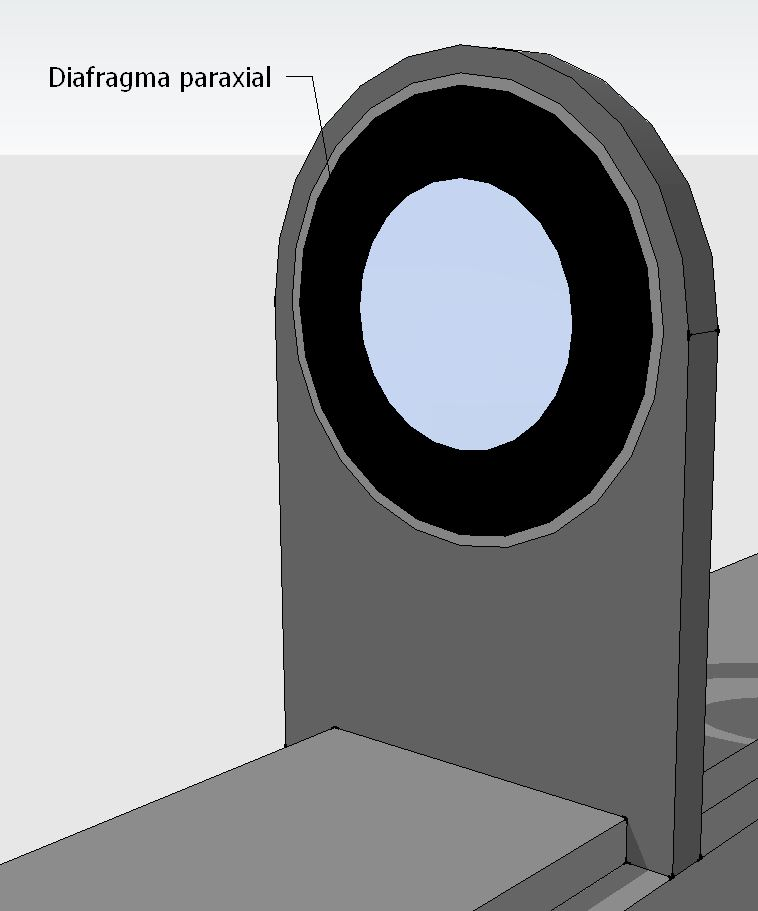
\includegraphics[width=0.7\linewidth]{DiafragmaParaxial.jpg}
            \captionof{figure}{Diafragma paraxial}
            \label{f: Dparax}
        \end{Figure}

        \begin{Figure}
            \centering
            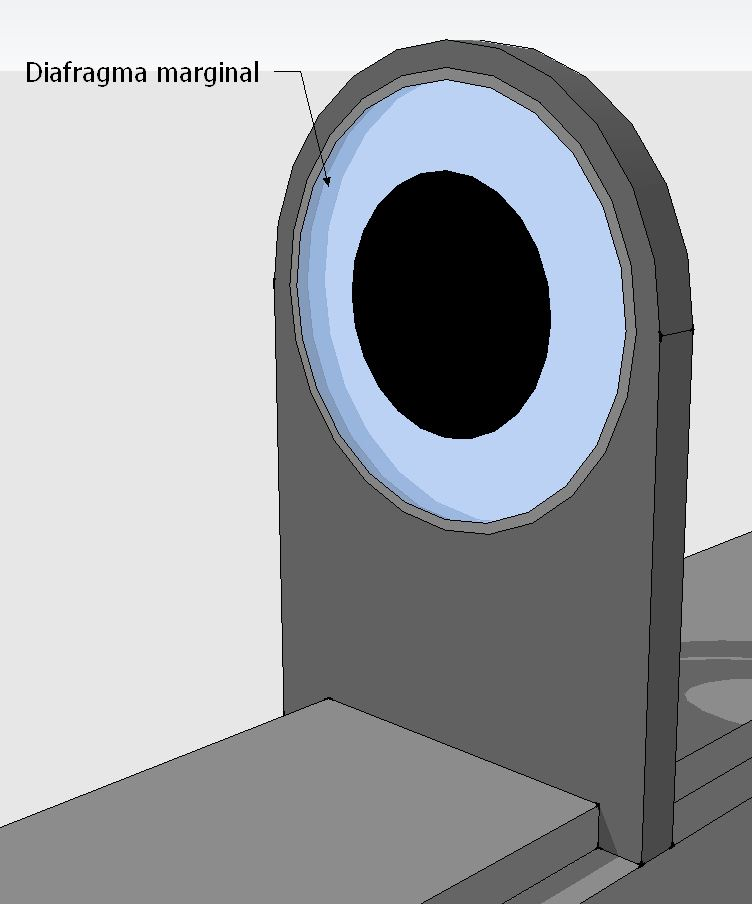
\includegraphics[width=0.7\linewidth]{DiafragmaMarginal.jpg}
            \captionof{figure}{Diafragma periférico}
            \label{f: Dmarg}
        \end{Figure}

        Las aberraciones de esfericidad y cromáticas van a ser despreciables si se cumple la ecuación \ref{eq:error}, que indica que bajo nuestras incertidumbres experimentales, no somos capaces de apreciar una diferencia entre las dos medidas que comparamos. Este control se realizó con la distancia focal del color rojo y del azul para el caso de aberraciones cromáticas. Mientras que para las aberraciones de esfericidad utilizamos la distancia focal con el diafragma paraxial y con el diafragma periférico.

        \begin{equation}
            \centering
            \Delta f_{a} + \Delta f_{r} \geq \abs{f_{a} - f_{r}}
            \label{eq:error}
        \end{equation}
 
        \begin{Figure}
            \centering

            \begin{tabular}{c|c c}
                \toprule
                 & \textit{Dist. objeto} & \textit{Dist. imagen}\\
                 & \textit{$[mm]$} & \textit{$[mm]$}\\
                \midrule
                Diafragma & \multirow{2}{*}{$(263 \pm 2)$} & \multirow{2}{*}{$(187 \pm 3)$}\\
                paraxial & & \\
                Diafragma & \multirow{2}{*}{$(256 \pm 8)$} & \multirow{2}{*}{$(19 \pm 1)\times 10$}\\
                periferico & & \\ \hline
                Rojo & $(255 \pm 6)$ &$(186 \pm 7)$\\
                Azul & $(253 \pm 5)$ &$(187 \pm 6)$\\ 
                \bottomrule
            \end{tabular}

            \captionof{table}{Dist. objeto e imagen para el control de supuestos}
            \label{tab:supuestos}
        \end{Figure}

        Recogemos los datos de la distancia imagen y la distancia objeto con una lente convergente en la zona de validez del modelo experimental. Estos datos están en la tabla \ref{tab:supuestos} y al utilizar la ecuación \ref{eq:1/i+1/o}, obtenemos los valores de las distintas distancias focales (tabla \ref{tab:DistFocalAb}), de donde podemos ver que bajo nuestras incertidumbres experimentales cumplimos los supuestos del modelo que utilizamos.

        \begin{Figure}
            \centering
            \begin{tabular}{c|c}
                \toprule
                            & \textit{Distancia focal}        \\
                            & \textit{$[mm]$}                 \\
                \midrule
                Diafragma   & \multirow{2}{*}{$(108 \pm 1)$} \\
                paraxial    &                                 \\
                Diafragma   & \multirow{2}{*}{$(109 \pm 5)$}  \\
                periferico  &                                 \\ \hline
                Rojo        & $(107 \pm 3)$                   \\
                Azul        & $(107 \pm 3)$                   \\ 
                \bottomrule
            \end{tabular}

            \captionof{table}{Dist. focales para el control de supuestos}
            \label{tab:DistFocalAb}
        \end{Figure}

\section*{Conclusiones}
    
    Dentro de las incertidumbres de nuestro sistema experimental, obtuvimos una correspondencia con el modelo de las lentes delgadas tanto para la lente convergente como para la lente divergente. Al comprobar tal correspondencia pudimos obtener los valores de distancia focal, que luego al compararlos con el valor brindado por el fabricante aseguramos que son iguales dentro de nuestras incertidumbres.
  
    Al utilizar el dispositivo PASCO para diseñar los sistemas experimentales se pudo reducir problemas prácticos como la linealidad del experimento, que podrían ser fuente de errores sistemáticos. La fuente de error mas grande del sistema es el intervalo de nitidez de las imágenes formadas en la pantalla, una propuesta para reducir el intervalo es el uso de diafragmas para las mediciones.
    

\begin{thebibliography}{99}

    \bibitem{1} Hecht, Zajac. 2003. \emph{Óptica}, 4th ed. Pearson Education.
    \bibitem{1} Jenkins, White. 1964. \emph{Fundamentos de óptica}, 3th ed. Aguilar S.A.
    \bibitem{1} Sears, Zemansky. 2018. \emph{Física universitaria}, vol. 2, 14th ed. Pearson Education.
    \bibitem{1} Serway, Jewett. 2004. \emph{Physics for Scientists and Engineers}, vol. 2, 6th ed. Brooks Cole.

\end{thebibliography}
%iker te la re comes doblada, sos alto gil. vos tambien belen, que miras
\end{multicols*}

\end{document}